\documentclass[tikz,border=10pt]{standalone}
\usepackage{amsmath,amssymb}
\usepackage{tikz}
\usepackage{pgfplots}
\pgfplotsset{compat=1.18}
\usetikzlibrary{arrows.meta,calc,patterns,positioning,shapes,decorations.markings,backgrounds,fit,intersections}

% Atlas colors
\definecolor{AtlasTeal}{HTML}{5BA4A4}
\definecolor{AtlasTealDark}{HTML}{4A8F8F}
\definecolor{AtlasTealLight}{HTML}{E8F4F4}
\definecolor{AtlasDeep}{HTML}{2C5F5F}
\definecolor{AtlasSage}{HTML}{7BAE7F}
\definecolor{AtlasSageLight}{HTML}{EDF5EE}
\definecolor{AtlasWarm}{HTML}{D4A853}
\definecolor{AtlasWarmLight}{HTML}{FDF6E8}

\begin{document}
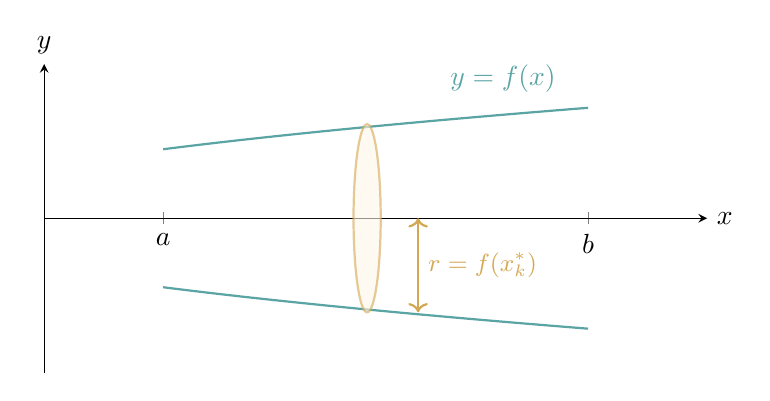
\begin{tikzpicture}
  \begin{axis}[
    width=10cm, height=5.5cm,
    axis lines=middle,
    xlabel={$x$}, ylabel={$y$},
    xtick={1,3.5}, xticklabels={$a$,$b$},
    ytick=\empty,
    xmin=0.3, xmax=4.2, ymin=-2, ymax=2,
    every axis x label/.style={at={(ticklabel* cs:1)}, anchor=west},
    every axis y label/.style={at={(ticklabel* cs:1)}, anchor=south},
  ]
    % Upper curve
    \addplot[AtlasTeal, thick, samples=100, domain=1:3.5] 
      {sqrt(0.5*x + 0.3)};
    % Lower curve (reflection)
    \addplot[AtlasTeal, thick, samples=100, domain=1:3.5] 
      {-sqrt(0.5*x + 0.3)};
    % A single disk (ellipse)
    \draw[AtlasWarm, thick, fill=AtlasWarmLight, opacity=0.6] 
      (axis cs:2.2,0) ellipse [x radius=0.08, y radius=1.22];
    % Annotations
    \draw[<->, thick, AtlasWarm] (axis cs:2.5,-1.22) -- 
      node[right, font=\small] {$r = f(x_k^*)$} (axis cs:2.5,0);
    \node[above, AtlasTeal] at (axis cs:3,1.5) {$y = f(x)$};
  \end{axis}
\end{tikzpicture}
\end{document}
